\documentclass{article}
\usepackage{graphicx}
\usepackage{booktabs}
\usepackage{parskip}
\usepackage{tcolorbox}
\usepackage[fleqn]{amsmath}
\usepackage{multicol}
\usepackage{amsmath}
\usepackage{multicol}
\usepackage{float}
\usepackage{amssymb}
\usepackage{gensymb}
\usepackage[inline]{enumitem}
\usepackage{titling}
\usepackage[margin=0.5in]{geometry}
\setlength{\droptitle}{-1in}
\usepackage{array}
\usepackage{amsmath}
\usepackage{natbib}
\usepackage{hyperref}
\newcommand{\commandnote}[1]{
    \begin{tcolorbox}[
        standard jigsaw,
        title=Note,
    ]
        #1
    \end{tcolorbox}
}
\newcommand{\minititle}[1]{
\subsubsection*{#1}
}

\title{\vspace{1ex} Data Eng. Notes \vspace{-1ex}}
\author{ibrahim.nasser@fau.de}
\date{}
\begin{document}
\maketitle
\section*{Disclaimer}

These are my personal notes and are not official course documents. They may contain inaccuracies or omissions, hence, they should not be considered as a substitute for official course materials or as comprehensive preparation for examinations.

\section*{Introduction and Basic Data Types}
We call the data \textbf{Tabular} when there are no modelled dependencies between attributes, for example, demographic attributes such as age, gender, ZIP code, etc. (also called \textit{Nondependency-Oriented Data}). Otherwise it is \textbf{Non-Tabular}, e.g. social networks, time series, etc.

\textbf{Matrix Representation of Data}

A set  $X = \{ X_i \mid  i \in \{1 \dots n \}\}, $ with $n$ records (samples) is a $d$-dimensional dataset iff each sample $X_i$ is a set of $\{ x_j \mid j \in \{ 1 \dots d\} \}$ attributes (features). $X$ is tabular if it is invariant w.r.t shuffling of samples and features. Each feature $x_j$ has its own domain $\mathcal{D}_j$

\mydef{Quantitative vs. Categorical}{A variable $x$ is quantitative (numeric) if its domain $\mathcal{D}_x$ is numeric. Otherwise, Categorical.
\textit{Examples (Q): }age, weight, height, BMI, Date of Birth.
\textit{Examples (C): }name, gender, country, ZIP Code, weather, ID, day.}

\mydef{Nominal vs. Ordinal}{A categorical variable $x$ is ordinal if its domain $\mathcal{D}_x$ has a natural ordering. Otherwise, Nominal.
\textit{Examples (N): }weather, name, gender, country, ZIP, ID, day
\textit{Examples (O): }heat level, textual gpa.}

\mydef{Finite vs. Infinite}{A variable $x$ has a finite domain iff $|\mathcal{D}_x| = N , N \in \mathbb{N}$. Otherwise, Infinite.
\textit{Examples (F): }age (years), country, ZIP, ID, gender, day.
\textit{Examples (I): }BMI, height, Date of Birth.}

\commandnote{All categorical variables have finite domains, not the other way around.}

\mydef{Discrete vs. Cont.}{A Quantitative variable $x$ is continuous iff $\forall z,y \in \mathcal{D}_x \exists w \in \mathcal{D}_x, z<w<y$. Otherwise, Discrete.
\textit{Examples (D): }age (years, months, days, hours, etc).
\textit{Examples (C): }age (unitless, number), Date of Birth (point in cont. time), BMI.}

\commandnote{By \textbf{rounding} quantitative data, we can transform cont. domains into discrete ones.}
\commandnote{Age is quantitative finite discrete if it is computed as whole years, months, days, hours. However, it is quantitative infinite continuous it is computed as precise value including fractions}
\commandnote{Date of Birth is quantitative infinite continuous since it is a point in a continuous endless time}

\mydef{Binary}{We call a variable $x$ binary iff $|\mathcal{D}_x|=2$}

\mydef{Temporal}{We call a variable $x$ temporal iff $\mathcal{D}_x$ represents time points or intervals. \textit{Examples:} day, month, Date of Birth}

\mydef{Encoding}{Data Encoding refers to the technique of converting data into a form that allows it to be properly used by different systems.}

\mydef{Binning}{Binning is an encoding technique that is a function $f : \mathcal{D} \to \{1 \dots K\}$}

\mydef{Example: Equal-Width Binning}{Size (width) of each bin is calculated as $W = \frac{\text{Max}(x)-\text{Min}(x)}{K}$ where $K$ is the number of bins.} 

\minititle{One-Hot Encoding}
To mitigate the problem of label encoding for nominal variables.\\
\textbf{How?} Create a fixed-size vector with size = $|\text{unique}(x)|$, where each position corresponds to a unique category value. Assign a \texttt{1} to the position representing the category and \texttt{0}s elsewhere.

\textbf{Example:}
Suppose $\text{unique}(x) = \{\text{Red}, \text{Green}, \text{Blue}\}$

\begin{itemize}
    \item Red $\rightarrow$ [1, 0, 0]
    \item Green $\rightarrow$ [0, 1, 0]
    \item Blue $\rightarrow$ [0, 0, 1]
\end{itemize}

\commandnote{
    One-hot encoding avoids the problem of implying ordinal relationships.
    However, it increases dimensionality significantly, especially when the number of categories is large (curse of dimensionality).
}

\minititle{Cyclic Encoding}
Some categorical variables are \textit{ordinal} and have a natural \textit{cyclic} structure. A classic example is the months of the year:
\[
\mathcal{D}_x = \{\text{Jan}, \text{Feb}, \dots, \text{Dec}\}
\]

This variable has both an order (Jan $<$ Feb $<$ ... $<$ Dec) and a cyclic relationship (Dec is followed by Jan).

To encode this properly, we use the index \( i \) of each category in the ordered list, where \( i = 1, 2, \dots, k \), and \( k \) is the total number of categories.

\textbf{Encoding Function:}
\[
\text{enc}(c_i) = (x_i, y_i)
\]
\[
x_i = \cos\left(\frac{2\pi(i-1)}{k}\right),\quad y_i = \sin\left(\frac{2\pi(i-1)}{k}\right)
\]

This maps each category to a unique point on the unit circle, preserving both order and cyclicity.

\commandnote{
    Cyclic encoding is useful when the first and last categories are conceptually adjacent (e.g., December and January). This is not possible with standard label or one-hot encoding.
}
\textbf{Optional: Normalize to Unit Square}
\[
\text{enc}(c_i) = \left(\frac{x_i + 1}{2},\ \frac{y_i + 1}{2}\right)
\]
This scaled version maps points to the square $[0, 1] \times [0, 1]$, which can be useful when input normalization is required for machine learning models. Note that this transformation alters the original unit circle geometry.

\commandnote{
    Use raw unit circle encoding when preserving angular distance is important. Use the normalized version when the model expects features in the range $[0, 1]$.
}   

\minititle{Non-Tabular Data}
Such as Spatial data, images, time series, string, graphs.

A set $X = \{x_i \mid i \in \{1 \dots n\}\}$ is a $d$-dimensional \textbf{spatial} dataset with $n$ samples if each sample $x_i$ contains a set of $\{ x_j \mid j \in \{ 1 \dots d\} \}$  features AND each data point $x_{ij}$ is associated with a specific spatial location $l$.

A spatial location $l$ can be a point $(l_x, l_y) \in \mathbb{R}^2$ (2D spatial data) or $(l_x, l_y, l_z) \in \mathbb{R}^3$ (3D spatial data), etc.

\minititle{Tokenization (Character-Level)}

Tokenization is the process of converting raw text into smaller units called tokens. In character-level tokenization, each unique character from the corpus is treated as a token.

\textbf{Example:} Consider the corpus consisting of a single sentence:  
\texttt{"hi ai"}

\begin{itemize}
    \item Unique characters: \texttt{\{h, i, \space, a\}}  
    \item Assign token IDs: \texttt{h:0,\ i:1,\space:2,\ a:3}
    \item Tokenized sentence: \texttt{"hi ai"} $\rightarrow$ \texttt{[0, 1, 2, 3, 1]}
\end{itemize}

Each character in the sentence is replaced by its corresponding token ID.

\minititle{Graphs}

A graph is a mathematical structure used to model pairwise relations between objects.

\begin{itemize}
    \item A graph \( G \) is defined as \( G = (V, E) \), where:
    \begin{itemize}
        \item \( V \) is a set of \textit{vertices} (or \textit{nodes}).
        \item \( E \subseteq V \times V \) is a set of \textit{edges}.
    \end{itemize}
\end{itemize}

\textbf{Types of Graphs:}
\begin{itemize}
    \item \textbf{Undirected Graph:}  
    An edge \( (u, v) \in E \) implies a bidirectional connection:  
    \[
    (u, v) \in E \Rightarrow (v, u) \in E
    \]

    \item \textbf{Directed Graph (Digraph):}  
    Edges have direction:  
    \[
    (u, v) \in E \not\Rightarrow (v, u) \in E
    \]
\end{itemize}

\minititle{Graph Representations}

\textbf{Adjacency Matrix:}

A \( |V| \times |V| \) matrix \( A \), where:
\[
A[u][v] = 
\begin{cases}
1 & \text{if } (u,v) \in E \\
0 & \text{otherwise}
\end{cases}
\]

\begin{itemize}
    \item \textbf{Space consumption:} \( \mathcal{O}(|V|^2) \)
    \item \textbf{Edge access:} \( \mathcal{O}(1) \)
    \item \textbf{Neighbor iteration:} \( \mathcal{O}(|V|) \)
\end{itemize}

\textbf{Adjacency List:}

Each vertex \( u \in V \) maintains a list of its neighbors.

\begin{itemize}
    \item \textbf{Space consumption:} \( \mathcal{O}(|V| + |E|) \)
    \item \textbf{Edge access:} \( \mathcal{O}(|V|) \) (worst-case search)
    \item \textbf{Neighbor iteration:} \( \mathcal{O}(\deg(u)) \), where \( \deg(u) \) is the degree of vertex \( u \)
\end{itemize}

    \textbf{Weighted Graphs:}  

    In some graphs, each edge \( (u, v) \in E \) is associated with a numerical value called a \textit{weight}, often representing cost, distance, capacity, etc.
    
    \begin{itemize}
        \item For weighted graphs, the edge set becomes:  
        \[
        E \subseteq V \times V \times \mathbb{R}
        \]
        or we define a weight function:  
        \[
        w : E \rightarrow \mathbb{R}
        \]
        \item In the adjacency matrix, \( A[u][v] \) stores the weight instead of a binary 0 or 1.
        \item In the adjacency list, each neighbor can be stored along with its edge weight as a tuple: \( (v, w(u, v)) \).
    \end{itemize}   
\newpage
\section*{Conceptual Modeling}
\mydef{ER Model}{Entity-Relationship Model is a high-level, conceptual framework to describe entities, their attributes, and the relationships between them.
}

\mydef{Entity}{Basic concept of the Entity-Relationship (ER) model. It is an object in the real world. E.g. e1 (some employee).}

\mydef{Attribute}{Entities have attributes that are the properties that describe them.}

\mydef{Entity Type}{All entities that have the same entity type share the same attributes. E.g. EMPLOYEE (type), e1 (Entity).}

\mydef{Attribute Value}{A particular entity has a specific value for each of its attributes.}

\mydef{Composite}{An attribute is composite if it is described in terms of its smaller parts. E.g. Name, some databases consider name as a composite attribute consisting of two \textbf{atomic} attributes First Name and Last Name.}

\mydef{Atomic/Simple}{Cannot be divided into smaller parts.}

\commandnote{
    These days, we store \textbf{date} as a single value attribute of the type \textit{DATE}. Earlier, date was considered as a composite attribute consisting of atomic attributes \textit{day, month, year}.
}

\mydef{Derived}{An attribute is derived if its value is calculated using other \textbf{stored} attributes, e.g. age.}

\mydef{Stored}{An attribute is stored if it cannot be derived from other attributes.}

\commandnote{
    Age is both derived and atomic. DateOfBirth is both composite and stored.
}

\mydef{Single-Valued}{An attribute is single-valued if it can have only one value. E.g. DateOfBirth is single-valued composite. Biological sex is single-valued atomic.}

\mydef{Multi-Valued}{An attribute is multivalued if it can have several values. E.g. college degrees is multivalued atomic and can have BSc, MSc, BEng, etc.}

\commandnote{
    Affiliation of an entity type RESEARCHER is multivalued (because one can have different affiliations) and composite because an affiliation could be represented as (Org. Name, Dept., Address, Role, Start Date, End Date).
}

\mydef{Entity Set}{Collection of entities of a particular entity type in a database in a given time point.}

\begin{tabular}{|l|l|} \hline
    Entity Type & Blueprint/Description \\ \hline
    Entity Set & Actual set of entities (entity instances) at a point in time \\ \hline
\end{tabular}
\commandnote{
    In ancient logic and philosophy we refer to the definition or conceptual content of a term as an \textit{intension}. However, the set of actual things that satisfy a concept is called \textit{extension}. Hence, Entity Type is called intension, Entity Set is called extension.
}

\mydef{Candidate Key (Key Attribute)}{A candidate key is an attribute (or set of attributes) that \textbf{uniquely} and \textbf{minimally} identifies each entity in an entity set. E.g. StudentID, studentEmail.}

\mydef{Primary Key}{A primary key is the chosen candidate key that will be used to uniquely identify entities in the database.}

\mydef{Foreign Key}{A foreign key is an attribute in one table/entity that references the primary key of another table/entity.
It expresses a relationship between two entity sets.}

\mydef{Composite Primary Key}{A composite primary key is a primary key that consists of two or more attributes combined together to uniquely identify a record in a table. Neither attribute alone is sufficient to guarantee uniqueness — but together, they do.}

This is common in relationship tables, for example: enrollment relationship between students and courses (M:M):

\begin{tabular}{|l|l|l|} \hline
    StudentID & CourseID & Grade \\ \hline
    101&CS101&A \\ \hline
    101&MATH201&B \\ \hline
    102&CS101&B+ \\ \hline
\end{tabular}

\mydef{Weak Entity Types}{Entity types without key attributes.}

\mydef{Strong Entity Types}{Entity types with key attributes.}

\subsection*{Relations}
If we want to model 1:M or M:1 relations, we use the idea of foreign key (modeling the relation with single value attribute). Examples:

\begin{tabular}{|l|l|} \hline
    PersonID & PersonName \\ \hline
    1&Alice\\ \hline
    2&Bob \\ \hline
\end{tabular}
\begin{tabular}{|l|l|} \hline
    categoryID & categoryName \\ \hline
    1&Sport\\ \hline
    2&Science \\ \hline
\end{tabular}
\begin{tabular}{|l|l|l|} \hline
    catID & catName & ownerID \\ \hline
    1&Daisy&1\\ \hline
    2&Smart&2 \\ \hline
    3&Sweet&1 \\ \hline
\end{tabular}
\begin{tabular}{|l|l|l|} \hline
    articleID & title & categoryID \\ \hline
    1&title&1\\ \hline
    2&title&2 \\ \hline
    3&title&1 \\ \hline
\end{tabular}

We model M:M Relations by creating an entity representing that relation (usually with composite primary key).

\mydef{Relationship Type}{The definition / template / blueprint of the relationship}

\mydef{Relationship Instance}{A single actual link between entities.}

\mydef{Relationship Set}{The collection of all relationship instances at a given time.}

\mydef{Participation}{We say that entity types $E_1 \dots E_n$ participate in the \textbf{relationship type} $R$.}

\mydef{Relationship Degree}{Number of participating entity types in the relation. E.g. consider a relation SUPPLY that models which suppliers supply which projects and what parts are supplied, the degree here is 3 due the three entity types (SUPPLIER, PROJECT, PART).}

\mydef{Role Name}{The name describing the part an entity plays in a relationship.}
 
\mydef{Recursive Relationship}{A relationship where the same entity type participates more than once with different roles. E.g. SUPERVISION.}

\mydef{Cardinality Ratio}{Specifies the maximum number of entities of one type that can be associated with an entity of another type in a relationship. Examples ($E_1$ BINARY\_RELATION $E_2$):}

Let $E_1$ and $E_2$ be the sets of entities of type $E_1$ and $E_2$, respectively. Let $R \subseteq E_1 \times E_2$ be the binary relation between them: $R = \{ (e_1, e_2) \mid e_1 \in E_1,\ e_2 \in E_2 \}$
\begin{itemize}
    \item \textbf{1:1 }each entity of type $E_1$ can be related to at most one entity of type $E_2$ and vice versa
    \[
    \forall e_1 \in E_1, \quad |\{ e_2 \in E_2 \mid (e_1, e_2) \in R \}| \leq 1
    \]
    \[
    \forall e_2 \in E_2, \quad |\{ e_1 \in E_1 \mid (e_1, e_2) \in R \}| \leq 1
    \]
    \item \textbf{1:M }one entity of type $E_1$ can be related to many entities of type $E_2$. Each entity of type $E_2$ can be related to at most one entity of type $E_1$
    \[
        \forall e_1 \in E_1, \quad |\{ e_2 \in E_2 \mid (e_1, e_2) \in R \}| \geq 0
        \]
        \[
        \forall e_2 \in E_2, \quad |\{ e_1 \in E_1 \mid (e_1, e_2) \in R \}| \leq 1
    \]
    \item \textbf{M:1 }Inverse of \textbf{1:M }
    \[
        \forall e_1 \in E_1, \quad |\{ e_2 \in E_2 \mid (e_1, e_2) \in R \}| \leq 1
        \]
        \[
        \forall e_2 \in E_2, \quad |\{ e_1 \in E_1 \mid (e_1, e_2) \in R \}| \geq 0
    \]
    \item \textbf{M:M }many entities of type $E_1$ can be related to many entities of type $E_2$ and vice versa
    \[
        \forall e_1 \in E_1, \quad |\{ e_2 \in E_2 \mid (e_1, e_2) \in R \}| \geq 0
        \]
        \[
        \forall e_2 \in E_2, \quad |\{ e_1 \in E_1 \mid (e_1, e_2) \in R \}| \geq 0
    \]
\end{itemize}

\textbf{Total vs. Partial Participation}
\begin{itemize}
    \item \textbf{Total Participation of } $E_1$ in $R$ \\
    $\forall e_1 \in E_1, \ \exists e_2 \in E_2 : (e_1, e_2) \in R$  
    (Every entity of $E_1$ is related to at least one entity of $E_2$.)

    \item \textbf{Partial Participation of } $E_1$ in $R$ \\
    $\exists e_1 \in E_1: \forall e_2 \in E_2, (e_1, e_2) \notin R$  
    (There exists an entity in $E_1$ that does not participate in $R$.)
\end{itemize}

\textbf{Migrating attributes from relations to entities:}
\begin{itemize}
    \item 1:1 relationship types: Attributes can be migrated to either participating entity. (e.g. EMP MANAGES DEPT, start\_date)
    \item 1:N or N:1 relationship types: Attributes should be migrated to the entity that participates at most once. (e.g. EMP WORKS\_FOR DEPT, start\_date)
    \item M:N relationship types: Attributes cannot be migrated to the participating entities and must remain on the relationship itself.
\end{itemize}

\mydef{Identifying Relationships}{a special relationship where a weak entity is identified by its relationship with a strong entity. The weak entity cannot exist without the strong entity, and the relationship plays a crucial role in providing the weak entity with a composite key.}

\mydef{Existence Dependency}{A weak entity depends on the strong entity for its existence. It cannot exist without being related to a strong entity.}

\commandnote{
    A weak entity type has total participation in its identifying relationship. This means that every instance of the weak entity must be associated with at least one instance of the strong entity. If it doesn't, the weak entity doesn't exist ("existence dependency").
}
Example: 
\begin{itemize}
    \item Consider we have the following strong entities, customer, product.
    \item To manage orders, we have two entities, order, orderItem.
    \item Order is a strong entity since each order has its ID
    \item However, OrderItem entity can have OrderID, LineNumber, ProductID, quantity, price, discount, etc.
    \item In this case, OrderItem entity is a weak one, it cannot exist unless an order exists, therefore, the primary key is composite (OrderID, LineNumber)
\end{itemize}

\mydef{Min-Max Modeling}{Given an entity $E$ participating in Relation $R$. If at least \textit{min} and at most \textit{max} instances of $E$ must participate in $R$ with $\textit{min}>=0, \textit{max}>=1, \textit{max}>=\textit{min}$, then we say $E$ respects min-max constraint (\textit{min}, \textit{max}) w.r.t $R$.
}

\minititle{ER Diagram}

\begin{figure}[H]
    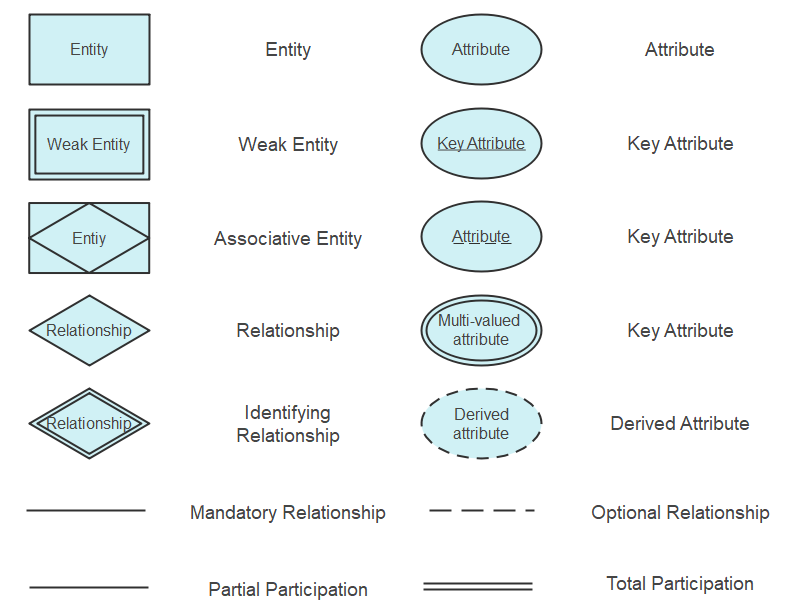
\includegraphics[width=0.4\linewidth]{images/chens-notation-1.png}
\end{figure}
\newpage
\section*{The Relational Data Model}
\mydef{Set}{
A set is a well-defined collection of distinct objects, considered as an object in its own right. The objects in a set are called elements or members. Sets are usually denoted by capital letters like $A$, $B$, or $S$, and elements are listed within curly braces. For example, $A = \set{1, 2, 3}$ is a set containing the numbers 1, 2, and 3.
}

\mydef{Element of a Set}{
If $x$ is an element of set $A$, we write $x \in A$. If $x$ is not in $A$, we write $x \notin A$.
}

\mydef{Set-builder Notation}{
Set-builder notation is a shorthand used to describe a set by stating the properties that its elements must satisfy.
For example: $\set{x \in \mathbb{N} \mid x \text{ is even} }$ describes the set of even natural numbers.
}

\mydef{Cardinality}{
The cardinality of a set is the number of elements in the set, denoted $|A|$.
For example, if $A = \set{1, 2, 3}$, then $|A| = 3$.
}

\mydef{Cartesian Product} {
Let $A$ and $B$ be sets, then $A \times B = \set{(a,b) \mid a \in A , b \in B}$, e.g. $A=\{1,2\}, B=\{x,y\}, A \times B = \set{(1,x),(1,y),(2,x),(2,y)}$
}

\mydef{Subset}{
$A\subseteq B \Leftrightarrow \forall X. X\in A \Rightarrow X \in B$
}

\mydef{Proper Subset}{
$A \subset B \Leftrightarrow A\subseteq B \land A \neq B$
}

\mydef{Relation}{
$R \subseteq A \times B$. If $(a,b) \in R$, we say that $a$ is related to $b$ via $R$
}

\mydef{Left Total Relation}{
A relation $R \subseteq A \times B$ is left total (total on $A$) iff each element in $A$ is related to at least on element in $B$. $\forall a \in A.  \exists b \in B. (a,b) \in R$
}

\mydef{Right Unique Relation}{
A relation $R \subseteq A \times B$ is right unique iff each element in $A$ is related to at most one element in $B$. $\forall a\in A, \forall b1, b2 \in B, ((a,b1) \in R,(a,b2)\in R) \Rightarrow b1 = b2$
}

\mydef{Function}{
A function is left total and right unique relation. $f:A \to B$
}

\mydef{Partial Function}{
A partial function is a right unique relation, \textbf{not} necessarily left total. $f \rightharpoonup B$
}

\mydef{Set Union}{
$x \in A \cup B \Leftrightarrow x \in A \text{ or }  x \in B$
}

\mydef{Set Intersection}{
$x \in A \cap B \Leftrightarrow x \in A \text{ and } x \in B$
}

\mydef{Disjoint}{
We say two sets $A,B$ are disjoint iff $A \cap B=\phi$
}

\mydef{Relation Schema}{A declaration $\textstyle R\bigl(A_1{:}D_1,\dots,A_n{:}D_n\bigr)$ consisting of a name $R$, a finite, non‑empty attribute set $\set{A_i}$ and, for each attribute, its domain $\operatorname{dom}(A_i)=D_i$.}

\mydef{Schema Satisfaction}{A \emph{tuple} $t=(v_1,\dots,v_n)$ \emph{satisfies} the schema if $v_i\in D_i\;\forall i$.}

\mydef{Types}{\textit{Classes} of atomic values that share representation and operations, e.g. \texttt{Int}, \texttt{Real}, or \texttt{String}.}

\mydef{Domain}{A \textit{set} of atomic values with application‑specific semantics whose underlying implementation type is fixed.  Domains may define default values.  Example: $\textit{EmployeeAge}=\texttt{Int}[18,65]$.}

\commandnote{Domain declaration examples: \texttt{Name = String(20)}, \texttt{DollarPrice = Decimal(5,2)}.}



\mydef{Instance}{A \emph{finite set} of tuples that all satisfy a given relation schema.  While the schema is comparatively stable (static), its instance is \emph{dynamic}: it evolves through insertions, deletions, and updates.}

\minititle{Two Equivalent Views on Tuples}

\begin{itemize}
    \item \textbf{Positional (Cartesian‑product) view:} $t$ is an \emph{ordered list} $\bigl(v_1,\dots,v_n\bigr)$.  Column order carries meaning; attribute names are implicit.
    \item \textbf{Functional view:} Fix $A=\set{A_1,\dots,A_n}$ and $D=\bigcup_i D_i$.  Then a tuple is a \emph{function} $t:A\to D$ with $t(A_i)\in D_i$.  Here, order is irrelevant and attribute names are explicit.
\end{itemize}

\mydef{Domain Constraint}{Each attribute value must lie in its declared domain $D_i$.  Usually enforced by the DBMS type checker.}

\mydef{Functional Dependency (FD)}{For attribute sets $X,Y\subseteq A$, the notation $X\to Y$ states: for any two tuples $t_1,t_2$, equality of $X$‑values implies equality of $Y$‑values.  Written out: $t_1[X]=t_2[X]\Rightarrow t_1[Y]=t_2[Y]$.}

\mydef{Superkey}{An attribute set $K$ with $K\to A$ (it functionally determines the whole tuple).}

\mydef{Candidate Key}{A \emph{minimal} superkey — removing any attribute from it destroys the functional determination of $A$.}

\mydef{Primary Key}{The candidate key chosen by the database designer to serve as the principal identifier of tuples in a relation.  Remaining candidate keys are called \emph{alternate keys}.}

% -- revised example ------------------------------------------------------
\minititle{Example}
\begin{itemize}
    \item Relation schema $\textit{Employee}(\textit{EmpID},\textit{SSN},\textit{Email},\textit{Name},\textit{Dept})$.
    \item \emph{Superkeys} include any attribute set that uniquely identifies tuples, e.g $\{\textit{EmpID}\},\;\{\textit{SSN}\},\;\{\textit{EmpID},\textit{Name}\}$. The third set still determines the whole tuple but is \emph{not} minimal.
    \item \emph{Candidate keys}: the minimal superkeys $\{\textit{EmpID}\}\quad\text{and}\quad\{\textit{SSN}\}$. Each is irreducible.
    \item \emph{Primary key}: suppose we designate $\textit{EmpID}$ as the primary key.  The other candidate becomes an \emph{alternate key} available for unique look‑ups.
\end{itemize}

\mydef{Foreign Key}{Attribute(s) in relation $R$ whose values must also appear as the primary-key values of another relation $S$ (ensuring referential integrity).}

\commandnote{When an insertion, deletion or modification would break any constaint, the DBMS may (i) reject the change or (ii) repair it automatically (``cascade'', insert default/null, etc.).  The exact behaviour is part of the schema definition.}
\end{document}

